
% Created by Bonita Graham
% Last update: December 2019 By Kestutis Bendinskas

% Authors: 
% Please do not make changes to the preamble until after the solid line of %s.

\documentclass[10pt]{article}
\usepackage[explicit]{titlesec}
\setlength{\parindent}{0pt}
\setlength{\parskip}{1em}
\usepackage{hyphenat}
\usepackage{ragged2e}
\RaggedRight

% These commands change the font. If you do not have Garamond on your computer, you will need to install it.
\usepackage{garamondx}
\usepackage[T1]{fontenc}
\usepackage{amsmath, amsthm}
\usepackage{graphicx}

\usepackage{listings}
\usepackage{mathtools}
\DeclarePairedDelimiter\ceil{\lceil}{\rceil}
\DeclarePairedDelimiter\floor{\lfloor}{\rfloor}

\usepackage{xcolor} % Define custom colours using \textcolor{color}{text}
\usepackage{float}

% Colour definitions
\definecolor{darkpink}{rgb}{1.0, 0.13, 0.32}

% This adjusts the underline to be in keeping with word processors.
\usepackage{soul}
\setul{.6pt}{.4pt}


% The following sets margins to 1 in. on top and bottom and .75 in on left and right, and remove page numbers.
\usepackage{geometry}
\geometry{vmargin={1in,1in}, hmargin={.75in, .75in}}
\usepackage{fancyhdr}
\pagestyle{fancy}
\pagenumbering{gobble}
\renewcommand{\headrulewidth}{0.0pt}
\renewcommand{\footrulewidth}{0.0pt}

% These Commands create the label style for tables, figures and equations.
\usepackage[labelfont={footnotesize,bf} , textfont=footnotesize]{caption}
\captionsetup{labelformat=simple, labelsep=period}
\newcommand\num{\addtocounter{equation}{1}\tag{\theequation}}
\renewcommand{\theequation}{\arabic{equation}}
\makeatletter
\renewcommand\tagform@[1]{\maketag@@@ {\ignorespaces {\footnotesize{\textbf{Equation}}} #1.\unskip \@@italiccorr }}
\makeatother
\setlength{\intextsep}{10pt}
\setlength{\abovecaptionskip}{2pt}
\setlength{\belowcaptionskip}{-10pt}

\renewcommand{\textfraction}{0.10}
\renewcommand{\topfraction}{0.85}
\renewcommand{\bottomfraction}{0.85}
\renewcommand{\floatpagefraction}{0.90}

% These commands set the paragraph and line spacing
\titleformat{\section}
  {\normalfont}{\thesection}{1em}{\MakeUppercase{\textbf{#1}}}
\titlespacing\section{0pt}{0pt}{-10pt}
\titleformat{\subsection}
  {\normalfont}{\thesubsection}{1em}{\textit{#1}}
\titlespacing\subsection{0pt}{0pt}{-8pt}
\renewcommand{\baselinestretch}{1.15}

% This designs the title display style for the maketitle command
\makeatletter
\newcommand\sixteen{\@setfontsize\sixteen{17pt}{6}}
\renewcommand{\maketitle}{\bgroup\setlength{\parindent}{0pt}
\begin{flushleft}
\sixteen\bfseries \@title
\medskip
\end{flushleft}
\textit{\@author}
\egroup}
\makeatother

% This styles the bibliography and citations.
%\usepackage[biblabel]{cite}
\usepackage[sort&compress]{natbib}
\setlength\bibindent{2em}
\makeatletter
\renewcommand\@biblabel[1]{\textbf{#1.}\hfill}
\makeatother
\renewcommand{\citenumfont}[1]{\textbf{#1}}
\bibpunct{}{}{,~}{s}{,}{,}
\setlength{\bibsep}{0pt plus 0.3ex}

\definecolor{mGreen}{rgb}{0,0.6,0}
\definecolor{mGray}{rgb}{0.5,0.5,0.5}
\definecolor{mPurple}{rgb}{0.58,0,0.82}
\definecolor{backgroundColour}{rgb}{0.95,0.95,0.92}

\setlength{\parindent}{0pt}

\lstdefinestyle{CStyle}{
    backgroundcolor=\color{backgroundColour},   
    commentstyle=\color{mGreen},
    keywordstyle=\color{magenta},
    numberstyle=\tiny\color{mGray},
    stringstyle=\color{mPurple},
    basicstyle=\footnotesize,
    breakatwhitespace=false,         
    breaklines=true,                 
    captionpos=b,                    
    keepspaces=true,                 
    numbers=left,                    
    numbersep=5pt,                  
    showspaces=false,                
    showstringspaces=false,
    showtabs=false,                  
    tabsize=2,
    language=C
}


%%%%%%%%%%%%%%%%%%%%%%%%%%%%%%%%%%%%%%%%%%%%%%%%%

% Authors: Add additional packages and new commands here.  
% Limit your use of new commands and special formatting.

% Place your title below. Use Title Capitalization.
\title{Final assignment ROS01}

% Add author information below. Communicating author is indicated by an asterisk, the affiliation is shown by superscripted lower case letter if several affiliations need to be noted.
\author{
Youri Klaassens$^{a}$, Nick van Endhoven$^{b}$ \\ \medskip 
$^{a}$student Computer Engineering Rotterdam University of Applied Science, 0996211@hr.nl, Zwaag \\ 
$^{b}$student Computer Engineering Rotterdam University of Applied Science, 0998831@hr.nl, Breda\\ \medskip 
}

\pagestyle{empty}
\begin{document}

% Makes the title and author information appear.
\vspace*{.01 in}
\maketitle
\vspace{.12 in}

% Introduction.
\section*{introduction}

This assignment considers a small part of a car; the airbag and blackbox system. The goal is to model
tasks so that all tasks reach their deadlines. The working platform is TI-RTOS. A second LaunchPad delivers the tasks to the main LaunchPad using 
GPIO pins. The tasks get executed and sent a signal back to the second LaunchPad. This second LaunchPad will then validate if the tasks are executed within their deadline.
The tasks and deadlines are defined in table \ref{tab:tasks}.

\begin{table}[H]
    \centering
    \begin{tabular}{|l|c|c|c|}
        \hline
        \textcolor{darkpink}{\textit{Task}}& \textcolor{darkpink}{\textit{Arrival time}} & \textcolor{darkpink}{\textit{BC deadline}} &  \textcolor{darkpink}{\textit{WC deadline}} \\
        \hline
        \textbf{Compass} & 200 ms $ \pm $ 20 ms & 5 ms & 35 ms \\
        \hline
        \textbf{Airbag} & 3000 ms $ \pm $ 1500 ms & 30 ms & 32 ms \\
        \hline
        \textbf{GPS} & 1300 ms $ \pm $ 20 ms & 5 ms & 70 ms \\
        \hline
    \end{tabular}

    \caption{Characteristics of the tasks. }
    \label{tab:tasks}
\end{table}

Table \ref{tab:pins} shows the pin mapping.

\begin{table}[H]
    \centering
    \begin{tabular}{|l|c|c|c|}
        \hline
        \textcolor{darkpink}{\textit{Description}}& \textcolor{darkpink}{\textit{Pin}} & \textcolor{darkpink}{\textit{GPIO}} &  \textcolor{darkpink}{\textit{IN/OUT}} \\
        \hline
        \textbf{Compass event} & 61 & 6 &  IN  \\
        \hline
        \textbf{Airbag event} & 62 &  7 &  IN  \\
        \hline
        \textbf{GPS event} & 63 & 8 &  IN  \\
        \hline
        \textbf{GPS response} & 64 & 9 &  OUT  \\
        \hline
        \textbf{Airbag response} & 1 & 10 &  OUT  \\
        \hline
        \textbf{Compass response} & 2 & 11 &  OUT  \\
        \hline
    \end{tabular}

    \caption{Pin mapping.}
    \label{tab:pins}
\end{table}

Both the \textit{compass} and \textit{GPS} tasks requires communication via a shared UART connection using 9600 baud 8N1 on UART0. The \textit{compass} task, on execution, has to print 32 bytes of ASCII data containing a counter
that increments every time the task is executed. The \textit{GPS} is required to do the same, but instead of 32 bytes it has to print 64 bytes of ASCII data.

\newpage
\section*{Implementation}

After the device is booted an initialization process is started. The UART and GPIO parameters are initialized and configured.
A main thread is created that summons different threads for each task with a given priority. Each of these
tasks are configured shown in listing \ref{lst:init}.

\begin{lstlisting}[style=CStyle, caption={Initialization}, captionpos=b, label={lst:init}, escapechar=@]
void* main_thread(void* args)
{
    struct sched_param  spc1, spc2, spc3;
    pthread_attr_t      pta_prio_1, pta_prio_2, pta_prio_3;
    pthread_t           ptc_c, ptc_a, ptc_g;

    check_errno( sem_init(&int_sem_compass, 0, 0) );
    check(pthread_attr_init(&pta_prio_1));
    check(pthread_attr_setstacksize(&pta_prio_1, 1024));
    check(pthread_attr_getschedparam(&pta_prio_1, &spc1));
    spc1.sched_priority = 1;
    check(pthread_attr_setschedparam(&pta_prio_1, &spc1));
    check(pthread_create(&ptc_c, &pta_prio_2, &compass_task, NULL));
    check_errno(pthread_join(ptc_c, NULL));
    check_errno( sem_destroy(&int_sem_compass) );
	
	...

    return NULL;
}

\end{lstlisting}

Each input GPIO pin gets its own callback function that will be executed on an interrupt. These interrupt are
enabled in the main before the main thread is created. Listing \ref{lst:events} shows these callback functions.
A semaphore is posted, respective to their task, when one of these events triggers. This allows the tasks
running in a different thread to continue execution. The way this implemented is shown in listing \ref{lst:tasks}.

\begin{lstlisting}[style=CStyle, caption={Interrupt callbacks}, captionpos=b, label={lst:events}, escapechar=@]
/* ISR for GPIO 06 */
void on_compass_event(uint_least8_t index)
{
    sem_post(&int_sem_compass);
}

/* ISR for GPIO 07 */
void on_airbag_event(uint_least8_t index)
{
    sem_post(&int_sem_airbag);
}

/* ISR for GPIO 08 */
void on_gps_event(uint_least8_t index)
{
    sem_post(&int_sem_gps);
}
\end{lstlisting}

In listing \ref{lst:tasks} also shows the implementation of the \textit{compass} task. When executed it writes a 32 byte ASCII
message using UART on baud 9600. This messages contains a counter, increased each execution, and fills the rest of the message with the character 'C'.
The \textit{GPS} tasks does the same thing but it writes a 64 byte message instead with the character 'G'. The function \texttt{write\_to\_uart} is shown in listing \ref{lst:uart}.
The \textit{airbag} task only has to wait for 30 ms before sending a signal bag.

\begin{lstlisting}[style=CStyle, caption={Tasks implementation}, captionpos=b, label={lst:tasks}, escapechar=@]
/* Task for compass */
void* compass_task(void* args)
{
    static int count = 0;

    while(1)
    {
        sem_wait(&int_sem_compass);

        write_to_uart(count, 'C', 32);

        count += 1;

        GPIO_write(Board_GPIO_11, 1);
        Task_sleep(1);
        GPIO_write(Board_GPIO_11, 0);
    }

    return NULL;
}
\end{lstlisting}

Since the UART resource has to be shared among two different threads a mutex lock is implemented. Each time a mutex will lock
the \texttt{UART\_write} function, preventing other threads from using it. This function is configured to be blocking, thus
only continuing after it finishes the writing process. After the function is fully executed
it will unlock again making it available for other threads to use. This is also shown in listing \ref{lst:uart}

\begin{lstlisting}[style=CStyle, caption={Write to UART implementation}, captionpos=b, label={lst:uart}, escapechar=@]
void write_to_uart(int cnt, char c, size_t size)
{
    char str[size];
    sprintf(str, "%d", cnt);

    int cnt_size = 0;
    int i = cnt;

    if(cnt == 0)
        cnt_size = 1;

    while(i != 0)
    {
        i /= 10;
        cnt_size += 1;
    }

    for(;cnt_size < size - 2; cnt_size++)
        str[cnt_size] = c;

    str[size - 3] = '\n';
    str[size - 2] = '\r';
    str[size - 1] = '\0';

    check_errno(pthread_mutex_lock(&uart_lock));
    UART_write(handle, str, size);
    check_errno(pthread_mutex_unlock(&uart_lock));
}
\end{lstlisting}

\newpage

\section*{Results}

Unfortunately we did not manage to get it fully working. Our program seems to unexpectedly crash
whenever the two threads try to enter the mutex locked area at around the same time. Figure \ref{resNoUART}
shows the results of the program without writing to UART.

\begin{figure}[H]
\caption{Result without shared UART resource}
\label{resNoUART}
\centering
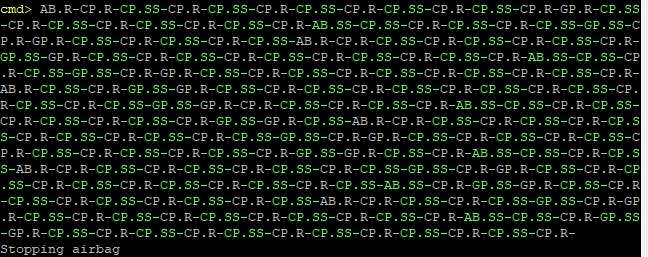
\includegraphics[width=0.9\linewidth]{./images/result_no_uart.jpeg}
\end{figure}

Figure \ref{res} shows the full results of the project with the \texttt{UART\_write} implementation.

\begin{figure}[H]
\caption{Result with shared UART resource}
\label{res}
\centering
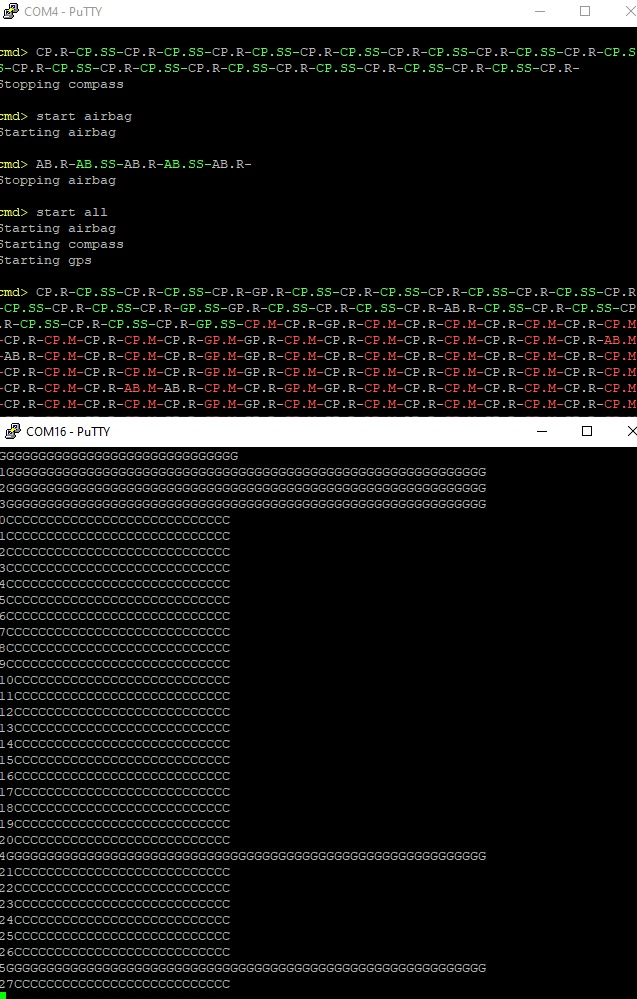
\includegraphics[width=0.9\linewidth]{./images/result.jpeg}
\end{figure}
\newpage

\section*{Conclusion}
\newpage
\end{document}
